
\begin{figure*}[tp!]
   \centering
   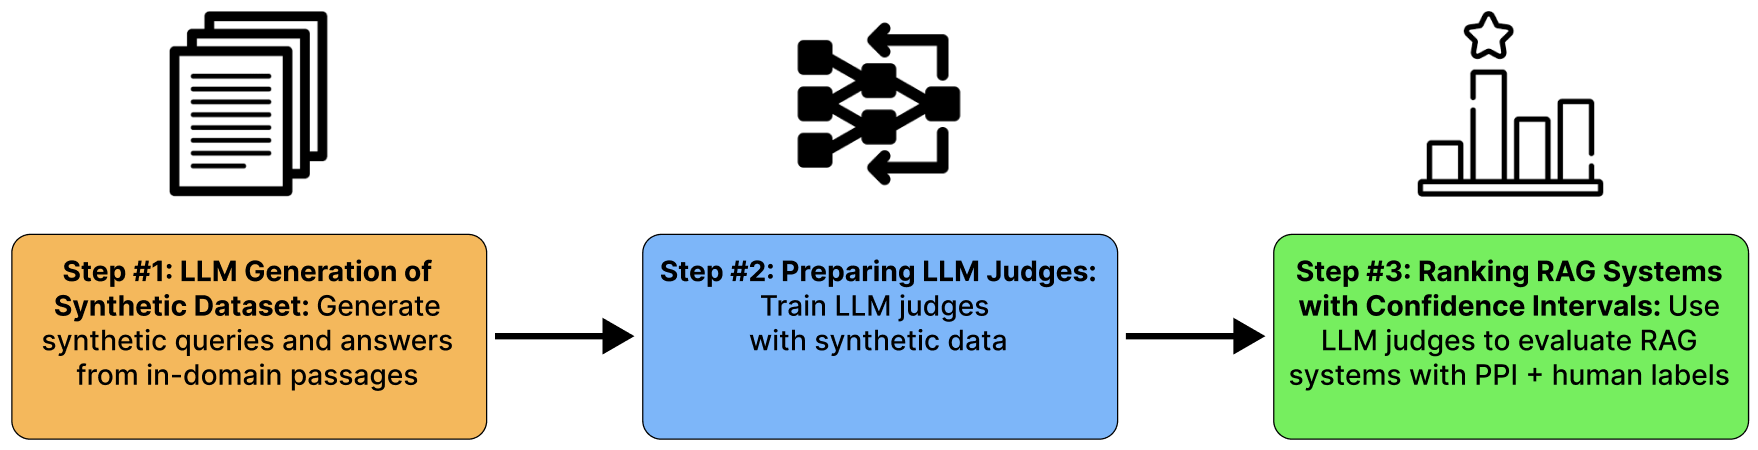
\includegraphics[width=0.9\linewidth]{Tables/Headline_Figure_V1.png}
   \caption{\textbf{Overview of ARES}:
   As inputs, the ARES pipeline requires an in-domain passage set, a human preference validation set of 150 annotated datapoints or more, and few-shot examples of in-domain queries and answers (five or more), which are used for prompting LLMs in synthetic data generation.
   To prepare our LLM judges for evaluation, we first generate synthetic queries and answers from the corpus passages. 
   Using our generated training triples and a constrastive learning framework, we fine-tune an LLM to classify query--passage--answer triples in three different criteria: context relevance, answer faithfulness, and answer relevance.
   Finally, we use the LLM judges to score RAG systems and generate confidence bounds for the ranking using PPI and the human preference validation set. 
   }
   \label{fig:domain_adaptation_diagram}
\end{figure*}



\section{ARES}
\label{sec:methods}




ARES proceeds in three stages (\autoref{fig:domain_adaptation_diagram}). 
There are three required inputs: an in-domain passage set, a human preference validation set of approximately 150 annotated datapoints (or more), and few-shot examples of in-domain queries and answers (five or more examples), which are used for prompting LLMs in synthetic data generation.
With our inputs prepared, we begin by generating synthetic queries (and their answers) from the passages in the target corpus. We then use these query--passage--answer triples to train LLM judges.
Subsequently, we apply these judges to any RAG system, scoring a sample of its in-domain query-document-answer triples, and use prediction-powered inference (PPI) with our human preference validation set to estimate a confidence interval for the quality of each RAG system.


\subsection{LLM Generation of Synthetic Dataset}

We generate synthetic queries and answers from the corpus passages using generative LLMs.
The generated data represent both positive and negative examples of query--passage--answer triples (e.g., relevant/irrelevant passages and correct/incorrect answers). 
For generation, the LLM uses our input set of few-shot examples with in-domain passages mapped to in-domain queries and answers; the model then generates a synthetic question and answer from a given in-domain passage, allowing us to create both positive and negative training examples. 
We include example prompts for generating synthetic queries and answers in \ref{sec:generate_synthetic_data}.

For creating our synthetic data, we primarily use on FLAN-T5~XXL (discussed in  \autoref{sec:models}). 
ARES works well with this model (see  \autoref{sec:results_and_analysis}) but our system can ultimately use another high-quality model for generating synthetic queries and answers.
We then filter out low-quality queries by testing if a given query can retrieve its original passage as the top result using its retriever.
This filtering approach has been used in previous work to isolate high-quality synthetic queries \cite{dai2022promptagator, saad2023udapdr}.

To generate negatives for fine-tuning our LLM judges, we rely on two novel strategies, generating the same number of negatives with each strategy:


\begin{enumerate}\setlength{\itemsep}{0pt}
    \item \textbf{Weak Negative Generation}: For context relevance negatives, we randomly sample in-domain passages unrelated to a given synthetic query. 
    For answer faithfulness and answer relevance negatives, we randomly sample synthetically-generated answers from other passages, which were created using FLAN-T5~XXL.
    \item \textbf{Strong Negative Generation}: For context relevance negatives, we randomly sample in-domain passages from the same document as the gold passage.
    For datasets in which multiple passages are not available for the same document, we use BM25 to retrieve the top-10 passages similar to the passage and sample from them for our context relevance strong negatives.  
    For answer faithfulness and answer relevance negatives, we prompt FLAN-T5 XXL (\autoref{sec:models}) to generate a contradictory answer using the few-shot prompt in \autoref{sec:flan_generate_synth_data}.
\end{enumerate}

In total, the number of negatives generated equals the number of positives generated for evaluating context relevance and answer relevance. %

\subsection{Preparing LLM Judges}

To prepare our RAG evaluation judges, we use our synthetic dataset to fine-tune DeBERTa-v3-Large judges (discussed in  \autoref{sec:models}) %
to evaluate %
three different capabilities
\cite{chen2023benchmarking, ragas2023}:

\begin{enumerate}\setlength{\itemsep}{0pt}
    \item \textbf{Context Relevance}: Is the passage returned relevant for answering the given query?
    \item \textbf{Answer Faithfulness}: Is the answer generated faithful to the retrieved passage, or does it contain hallucinated or extrapolated statements beyond the passage?
    \item \textbf{Answer Relevance}: Is the answer generated relevant given the query and retrieved passage?
\end{enumerate}

For each metric, a separate LLM with a binary classifier head is fine-tuned to classify positive and negative examples. 
For each concatenated query-document-answer, a single LLM judge must classify the triple as positive or negative for that judge's metric.
To fine-tune these judges, we use our human preference validation set to evaluate model improvement after each epoch, stopping when we have three epochs with no improvement in loss (see \autoref{sec:finetuning_configuration} for more information).



\subsection{Ranking RAG Systems with Confidence Intervals}
\label{sec:ranking_rag_with_ppi}

Once we have prepared our LLM judges, we need to use them to score and rank the competing RAG systems. 
To do this, ARES samples the in-domain query-document-answer triples produced by each RAG approach, and the judges label each triple, predicting their context relevance, answer faithfulness, and answer relevance.
By averaging the individual predicted labels for each in-domain triple, we calculate the RAG system performance across each of the three metrics.

In principle, we could simply report these average scores as quality metrics for each RAG system. However, these scores reflect entirely unlabeled data with predictions from a synthetically-trained LLM judge, and hence they may not be entirely accurate.
As an extreme alternative, we could use just the small human preference validation set discussed previously for evaluation, reporting the extent to which each RAG system agrees with (or deviates from) the human annotations.
However, an annotation-based evaluation approach would require labeling substantially more generative outputs from each RAG systems separately, which can be costly both in terms of time and financing.

To combine the benefits of both, and hence boost the precision of the evaluation, ARES uses \textit{prediction-powered inference} (PPI; \citealt{angelopoulos2023predictionpowered}) to predict the system scores. PPI is a recent statistical method that provides tighter confidence intervals on a small set of annotated datapoints (i.e., our validation set) by leveraging predictions on a much larger set of non-annotated datapoints.
PPI can leverage both the labeled datapoints and the ARES judge predictions on the non-annotated datapoints to construct confidence intervals for our RAG system's performance. %

To do this, PPI uses the LLM judges on the human preference validation set to learn a \textit{rectifier function} for constructing a confidence set of the ML model's performance, using each ML prediction in the larger non-annotated dataset. 
The confidence set can then be used to create a tighter confidence interval for the performance of the evaluated RAG system (e.g. its context relevance, answer faithfulness, or answer relevance accuracy individually) compared to simply using annotated outputs from the evaluated RAG system.
By bolstering the human preference validation set with the much larger set of datapoints with ML predictions, PPI can develop reliable confidence intervals for ML model performance that beat previous classical inference approaches.

The PPI rectifier function allows us to estimate the errors of the LLM judge and generate confidence bounds for the success and failure rates of the RAG system, estimating context relevance, answer faithfulness, and answer relevance performance.
Additionally, PPI allows us to estimate confidence intervals with a selected level of probability; for our experiments, we use a standard 95\% alpha (probability) for our confidence interval.

With the accuracy confidence interval for each component of the RAG, we find the midpoint of each confidence interval and use the midpoints to rank the RAG systems.
With our ranking, we can compare different RAG systems, as well as different configurations of the same RAG system, to find the best-performing approach for a given domain.
